
\newpage
\section{Full array fine tuning and results}

\begin{figure}[t] 
	\centering
	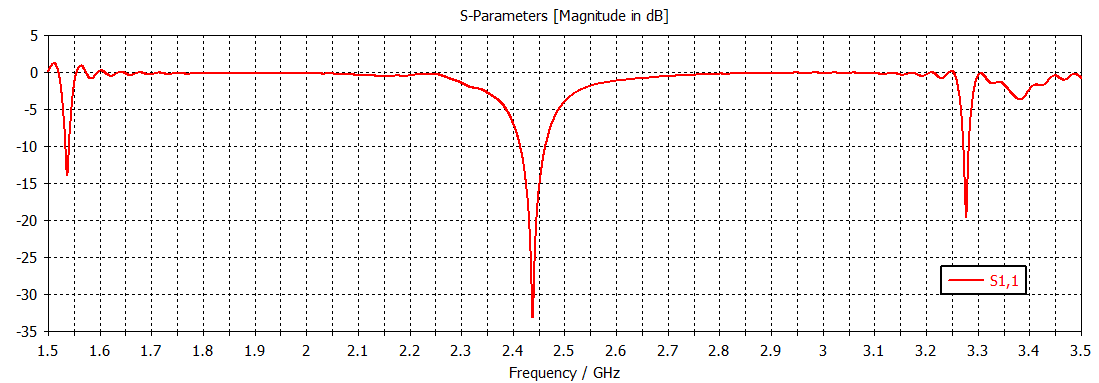
\includegraphics[scale=0.45]{p3_RL}
	\caption{Broadband view for the input reflection coefficient seen from full array input port.}
	\label{fig:p3_scattering}
\end{figure}
Within this last step the tuned BFN and radiating part are connected. The spacing between elements is set to be compliant with the GL limit at the central resonance frequency f\textsubscript{0}=2.45GHz (distance between elements, d=$\leq$88mm). 
Actually what follows mainly concerns the full antenna's radiation pattern, rather than the array factor alone. This is legitimated by the following facts:
\begin{itemize}
	\item what can be measured to describe the real radiation properties of a microstrip array antenna is the far field radiation pattern;
	\item the full AF's extraction from simulation introduces numerical errors that makes the calculation inaccurate far from the main lobe centre.
\end{itemize}
Furthermore,  moving the GL requirement from AF to the radiation patter, we gain a more robust design, less affected by discontinuities' and line width's losses\footnote{the total radiation pattern is given by the product of the single patch's pattern and the normalized array factor. Since the former term damps the latter then the total radiated field will be lowered as well. Moreover we can relax the requirement on tapering having more uniform microstrip lines (in terms of width).}.  

Patch's width and length are set equal to: W\textsubscript{patch}=64mm and L\textsubscript{patch}=24.7mm. Once BFN and radiators have been joint, we have the complete array reported in figure \ref{fig:p3_array}, which has been simulated with the mesh settings printed in figure \ref{fig:p3_mesh}. To keep the computation simpler we exploited the microstrip field distribution and a (y,z) transverse magnetic field symmetry plane has been used as boundary condition (with open boundary, added space in all directions).

Finally, the simulation's outcomes are the following:
\begin{description}
	\item[Return loss and bandwidth] Overall, the input reflection coefficient is worsened by the connection of the two parts. Although the various sections have been finely tuned, the difference between using excitation ideal port and connecting actual transmission lines cannot be reduced further. We reported in figure \ref{fig:p3_scattering} the best result allowed by optimization. Unfortunately $|$S\textsubscript{11}$|$ reaches its minimum at f\textsubscript{0}\textquotesingle=2.438GHz, not exactly at f\textsubscript{0}=2.45GHz. Though we obtained such discrepancy, this should not be a problem because this simulation does not represents the real behaviour of the built antenna, whose production is affected by technological limitations related to the quality of the chosen realization process (i.e. leading to fluctuation in the substrate dielectric permittivity, or consistency in line widths and lengths), that eventually leads to difference between simulated and actual antenna.  
	Besides that, the -20dB bandwidth is B\textsubscript{-20dB}=14.741MHz around f\textsubscript{0}\textquotesingle=2.438GHz, whereas  B\textsubscript{-10dB}=49.249MHz, this is a very selective (narrowband) antenna. To sum up, the array looks barely behaving as expected both in- and out-of-band, this must be confirmed by measurements though.
	
	\item[Far field radiation pattern] The radiation pattern (with cuts) and the axial ratio are depicted in figures from \ref{fig:p3_RP} to \ref{fig:p3_cuts2}. These pictures confirm that we have a broadside array (expected, since the radiators are positioned along the $x$-axis). The ground plane and the beam forming network presence distort the pattern, preventing the array to radiate along negative $y$-axis tilting the main lobe and directing the maximum radiation along ($\theta=-13^\circ$,$\varphi=90^\circ$).
	Moreover, from figure \ref{fig:p3_axial} we notice that the antenna is fully linearly polarized at least within the (y,z) plane (since the patch is single-edge fed this is a expected too). 
	
	\item [HPBW and SLL] From figure \ref{fig:p3_cuts2}b,c one has HPBW~=~20.4$^\circ$ and SLL=-20.7dB within the (y,z) plane.
\end{description}

\begin{figure}[t] 
	\centering
	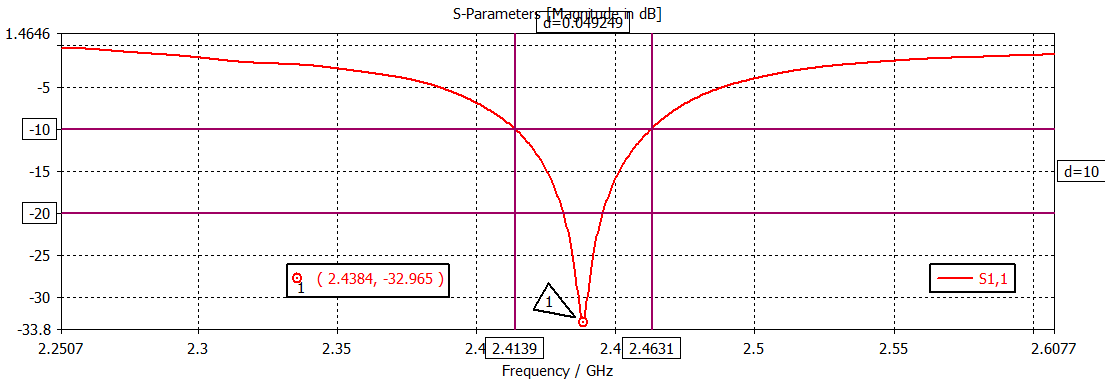
\includegraphics[scale=0.45]{p3_RL2}
	\caption{In-band view for the input reflection coefficient seen from full array input port.}
	\label{fig:p3_scattering_band}
\end{figure}

\begin{figure}[p] 
	\centering
	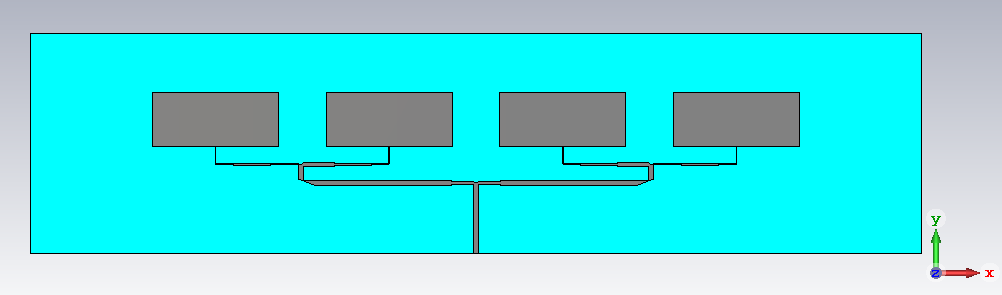
\includegraphics[scale=0.75, angle=90]{p3_array}
	\caption{Full array top view, (x,y) plane.}
	\label{fig:p3_array}
\end{figure}
\begin{figure}[p] 
	\centering
	\subfloat[][\emph{General settings}]{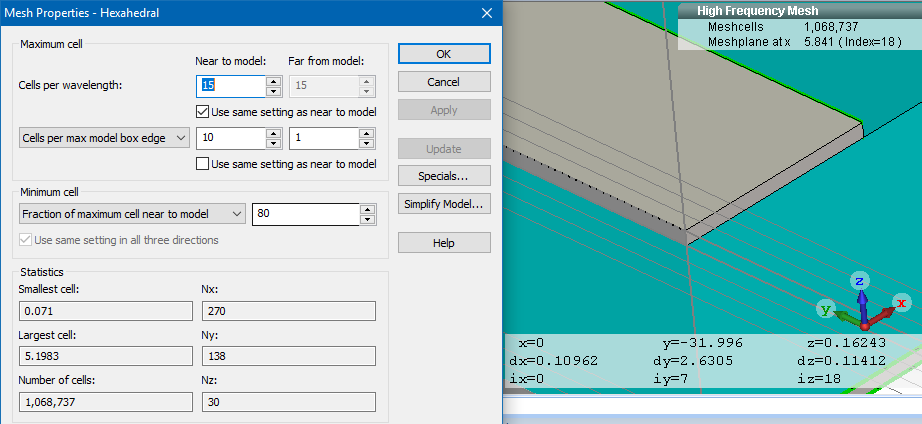
\includegraphics[scale=.5]{p3_mesh1}}\quad
	\subfloat[][\emph{Special settings}]{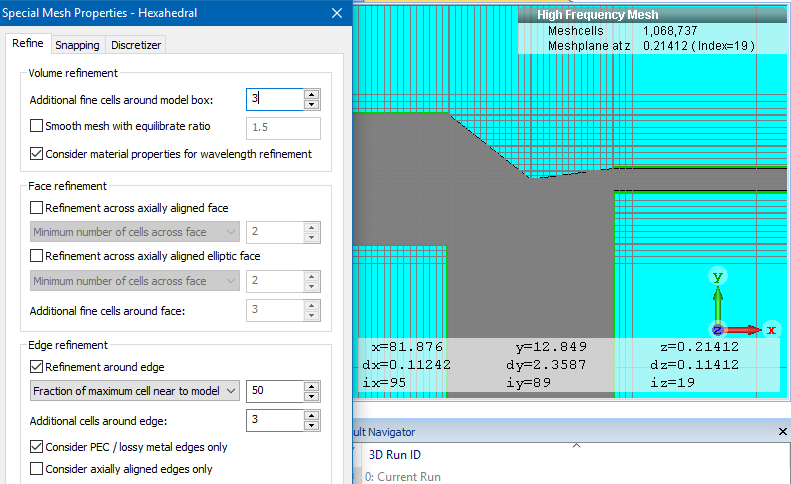
\includegraphics[scale=.5]{p3_mesh2}}\quad
	\subfloat[][\emph{Boundary conditions: symmetry plane}]{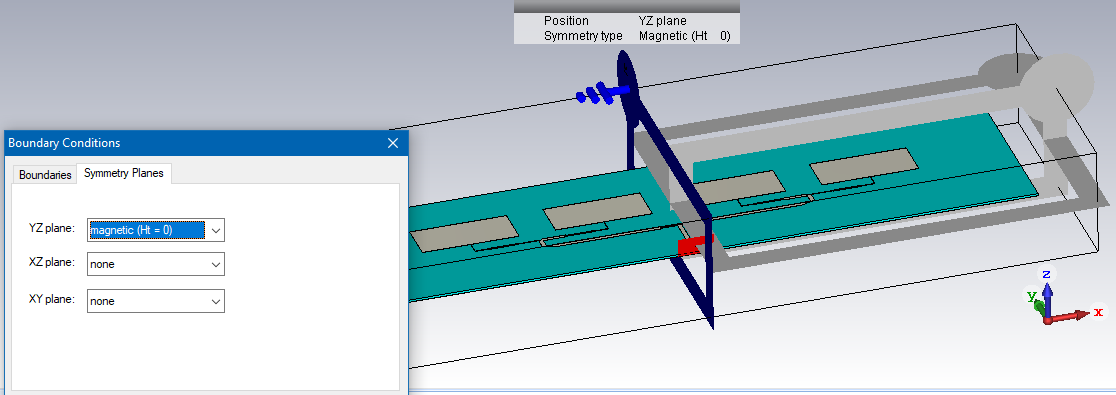
\includegraphics[scale=.4]{p3_JamesBonday}}\\
	\caption{Mesh general and special settings. As it appears the mesh has been increased to fit all the bends and narrower lines the best way.}.
	\label{fig:p3_mesh}
\end{figure}

\begin{figure}[p] 
	\centering
	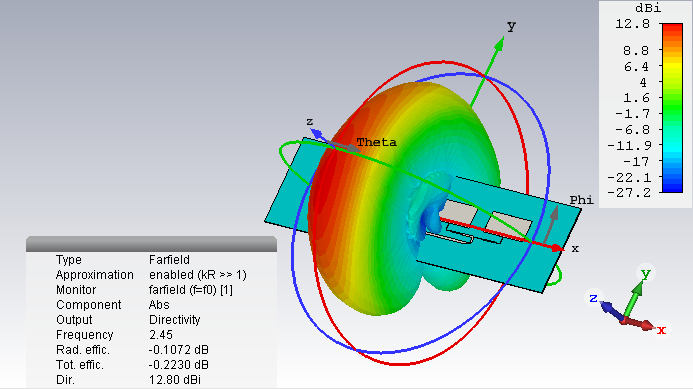
\includegraphics[scale=0.65]{p3_RP}
	\caption{3D far field radiation pattern.}
	\label{fig:p3_RP}
\end{figure}
\begin{figure}[p] 
	\centering
	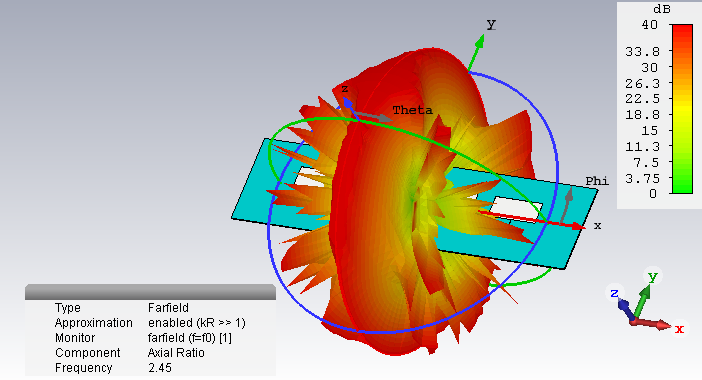
\includegraphics[scale=0.65]{p3_axial}
	\caption{Far field axial ratio.}
	\label{fig:p3_axial}
\end{figure}
\begin{figure}[p] 
	\centering
	\subfloat[][\emph{(x,y) plane cut, $\theta=0^\circ$}]{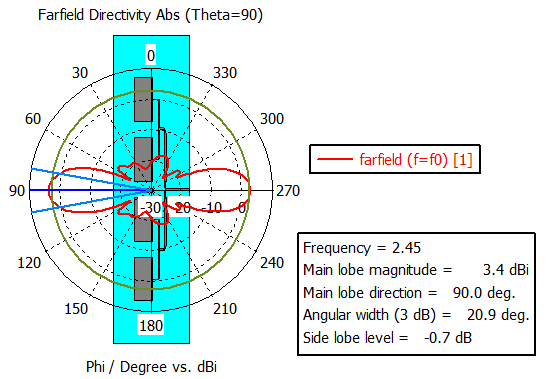
\includegraphics[scale=.7]{p3_XY}}\quad
	\subfloat[][\emph{(y,z) plane cut, $\varphi=0^\circ$}]{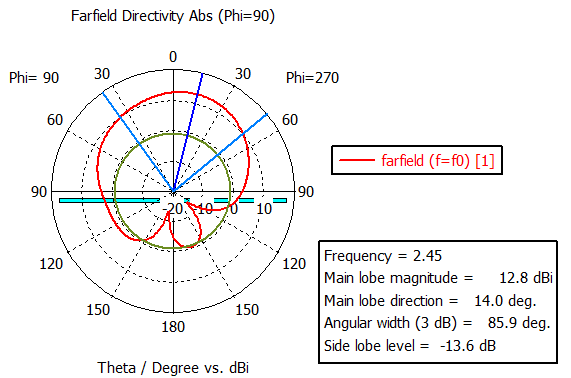
\includegraphics[scale=.7]{p3_YZ}}\\
	\caption{Radiation pattern's directivity polar cut planes. As it appears the array radiates broadside within the (y,z) plane. The radiation is minimum along the negative $y$-direction.}.
	\label{fig:p3_cuts1}
\end{figure}

\begin{figure}[p] 
	\centering
	\subfloat[][\emph{(x,z) plane polar cut,$\varphi=0^\circ$}]{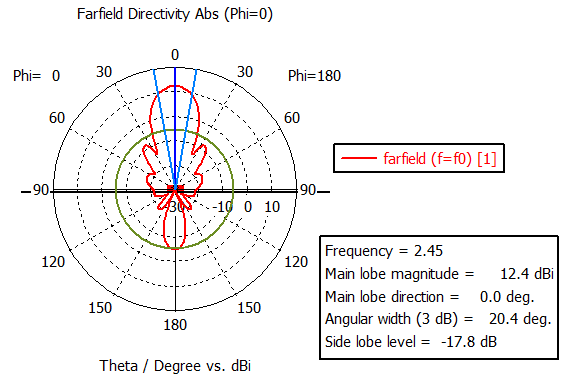
\includegraphics[scale=.7]{p3_XZ}}\quad
	\subfloat[][\emph{(x,z) plane cartesian view, $\varphi=0^\circ$}]{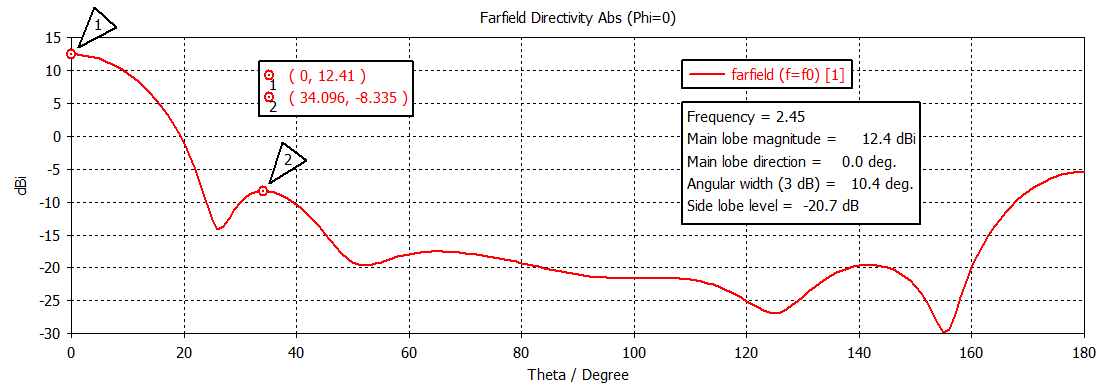
\includegraphics[scale=.4]{p3_XZ_cart}}\quad
		\subfloat[][\emph{positive (x,z) plane cartesian view, $\varphi=0^\circ$}]{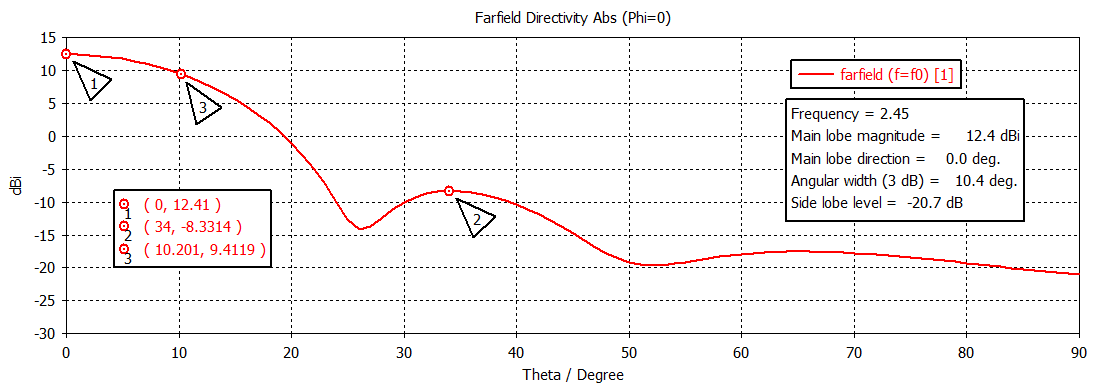
\includegraphics[scale=.4]{p3_XZ_cart2}}\\
	\caption{Radiation pattern's cut planes. As it appears the array radiates broadside within the (y,z) plane. The side lobes level limit is fulfilled, HPBW=20.4$^\circ$.}.
	\label{fig:p3_cuts2}
\end{figure}

\newpage 
\appendix
\section{Appendix: bends design}

Every time a bend is present, it introduces capacitive and inductive contributions to the microstrip line. To compensate this effects we varied the bend angle till the optimum is reached. To design the bend we cut away the highlighted part in figure \ref{fig:A_bend1}a, obtained by rotating by an angle $\alpha$ a rectangle then subtracted from the bend with boolean transformation. The simulation of the 50$\Omega$ bend within the 3dB splitter confirms the compensation (figure \ref{fig:A_bend}). Another relevant parameter is represented by the cut's position with respect to the bend's external corner, changed by means of the parameter a that can be found in figure \ref{fig:A_bend1}b. The input reflection coefficient variation is printed in figure \ref{fig:A_bend}. 

\begin{figure}[H] 
	\centering
	\subfloat[][\emph{cut's angle}]{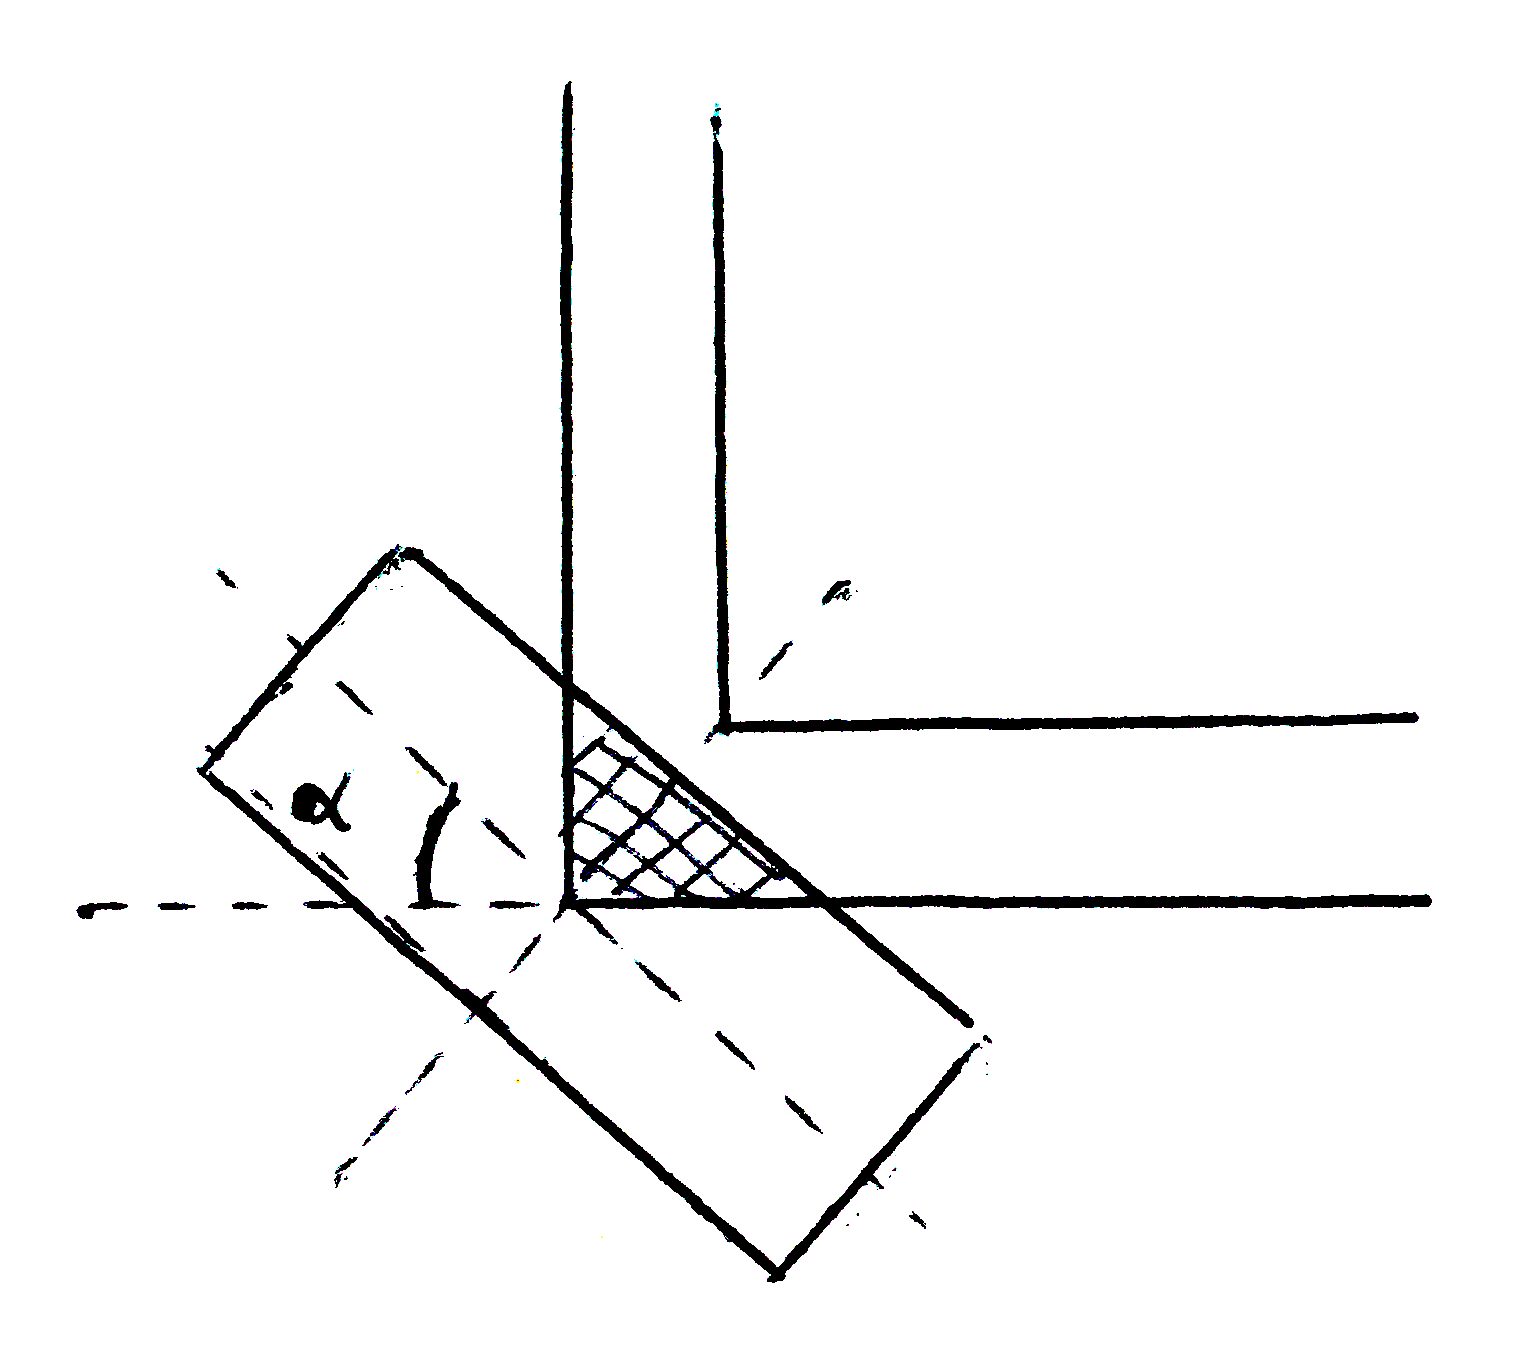
\includegraphics[scale=.5]{A_bends}}\quad
	\subfloat[][\emph{cut's position}]{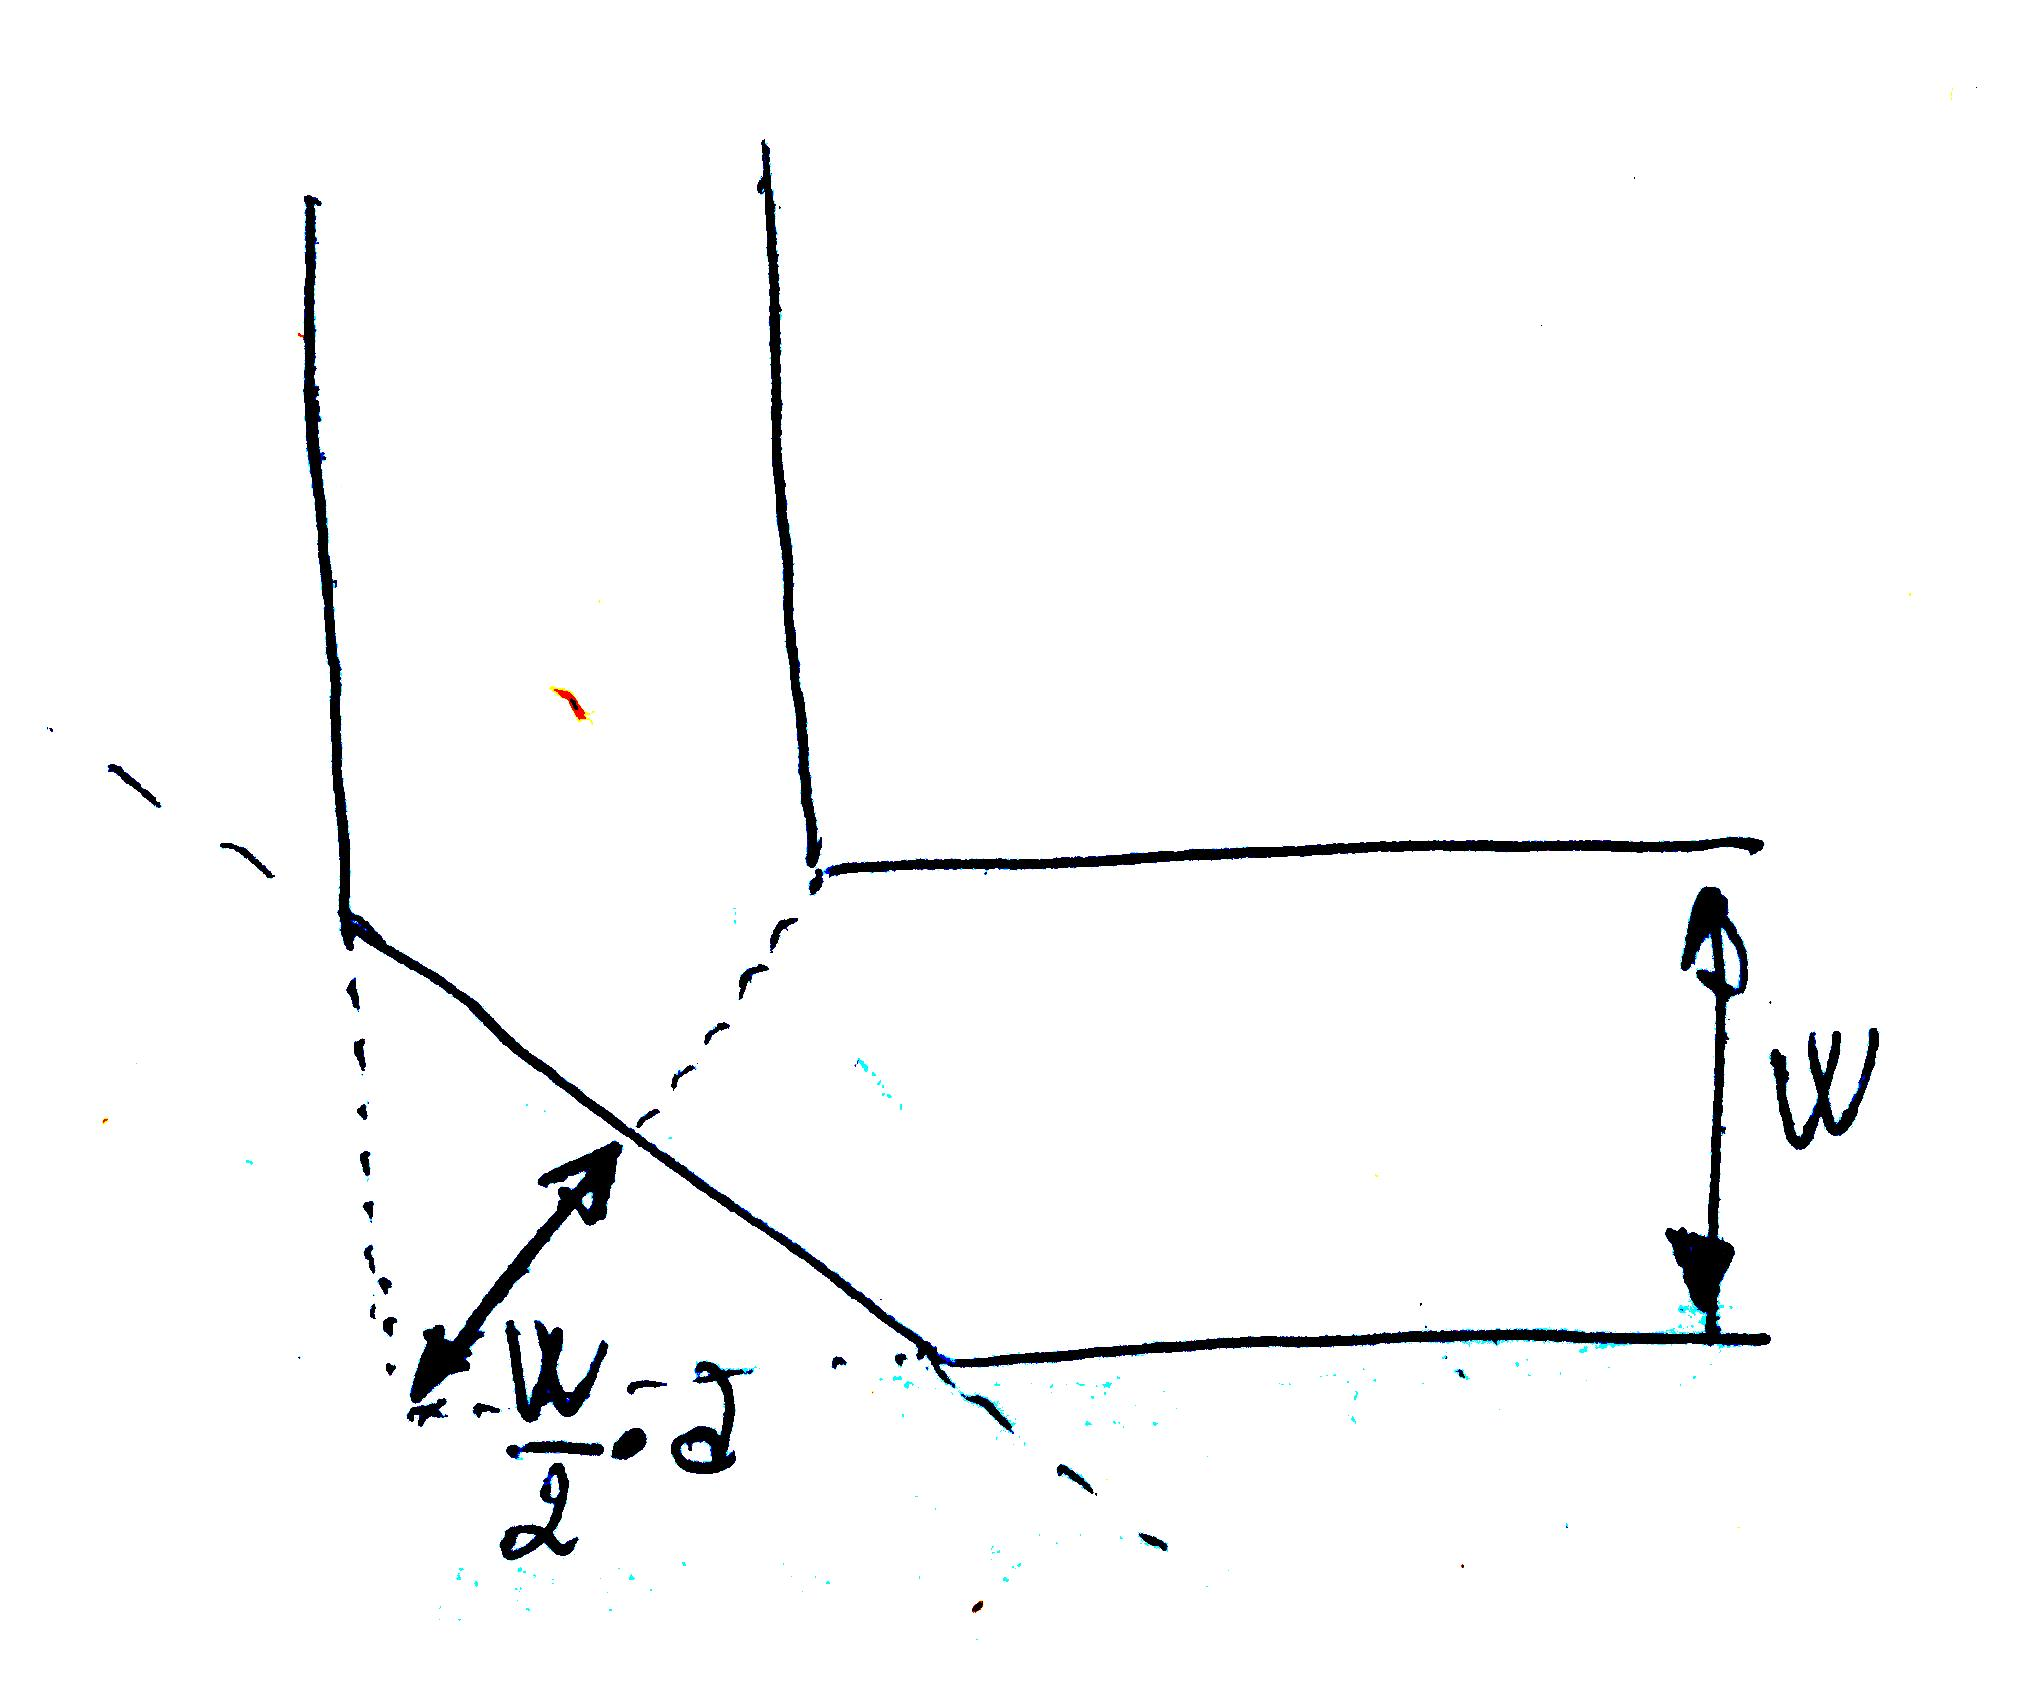
\includegraphics[scale=.4]{A_bends3}}\\
	\caption{Bend design}.
	\label{fig:A_bend1}
\end{figure}
 
 \begin{figure}[H] 
 	\centering
 	\subfloat[][\emph{sweep on $\alpha$}]{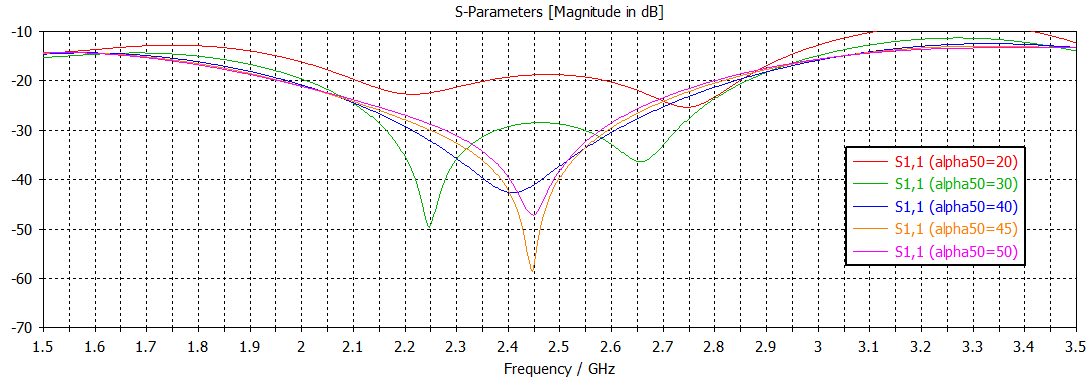
\includegraphics[scale=.3]{A_bends2}}\\
 	\subfloat[][\emph{sweep on a}]{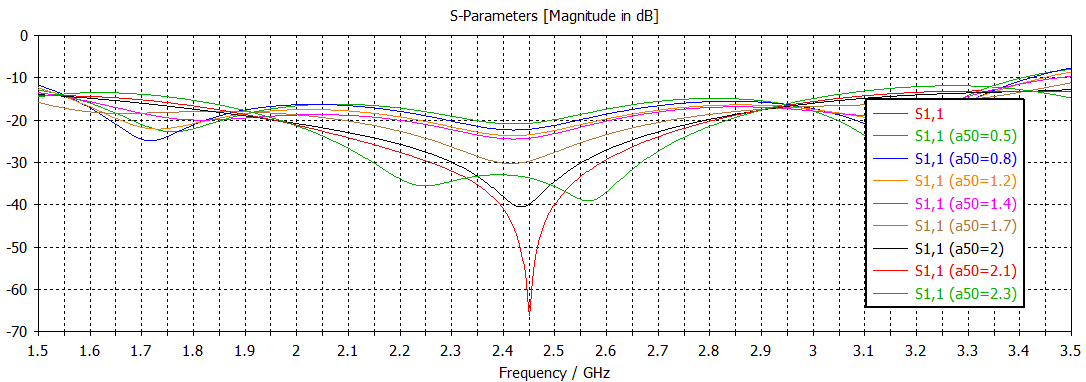
\includegraphics[scale=.3]{A_bends4}}\\
 	\caption{Input reflection coefficient varying bend's parameters.}.
 	\label{fig:A_bend}
 \end{figure}

\newpage 
\section{Appendix: mitered T-junction design}

Mitered junctions have been used to have better power splitting performance within the BFN. Looking at figure \ref{fig:p3_mitered_junctions}b one can notice that the cut is positioned with the aim of giving the power the same path length both toward left and right branch. Referring to figure \ref{fig:p3_mitered_junctions}a:
\begin{equation}
l = \sqrt{\Big(\frac{W_{50}}{2}\Big)^2+\Big(\frac{W_{70}}{2}\Big)^2} \notag
\end{equation}
and
\begin{equation}
\theta = \sin^{-1}\frac{1}{2}\frac{W_{70}}{l} \notag
\end{equation}
To design the section depicted in figure \ref{fig:p3_mitered_junctions}b the same calculations hold.

\begin{figure}[H] 
	\centering
	\subfloat[][\emph{3dB splitter}]{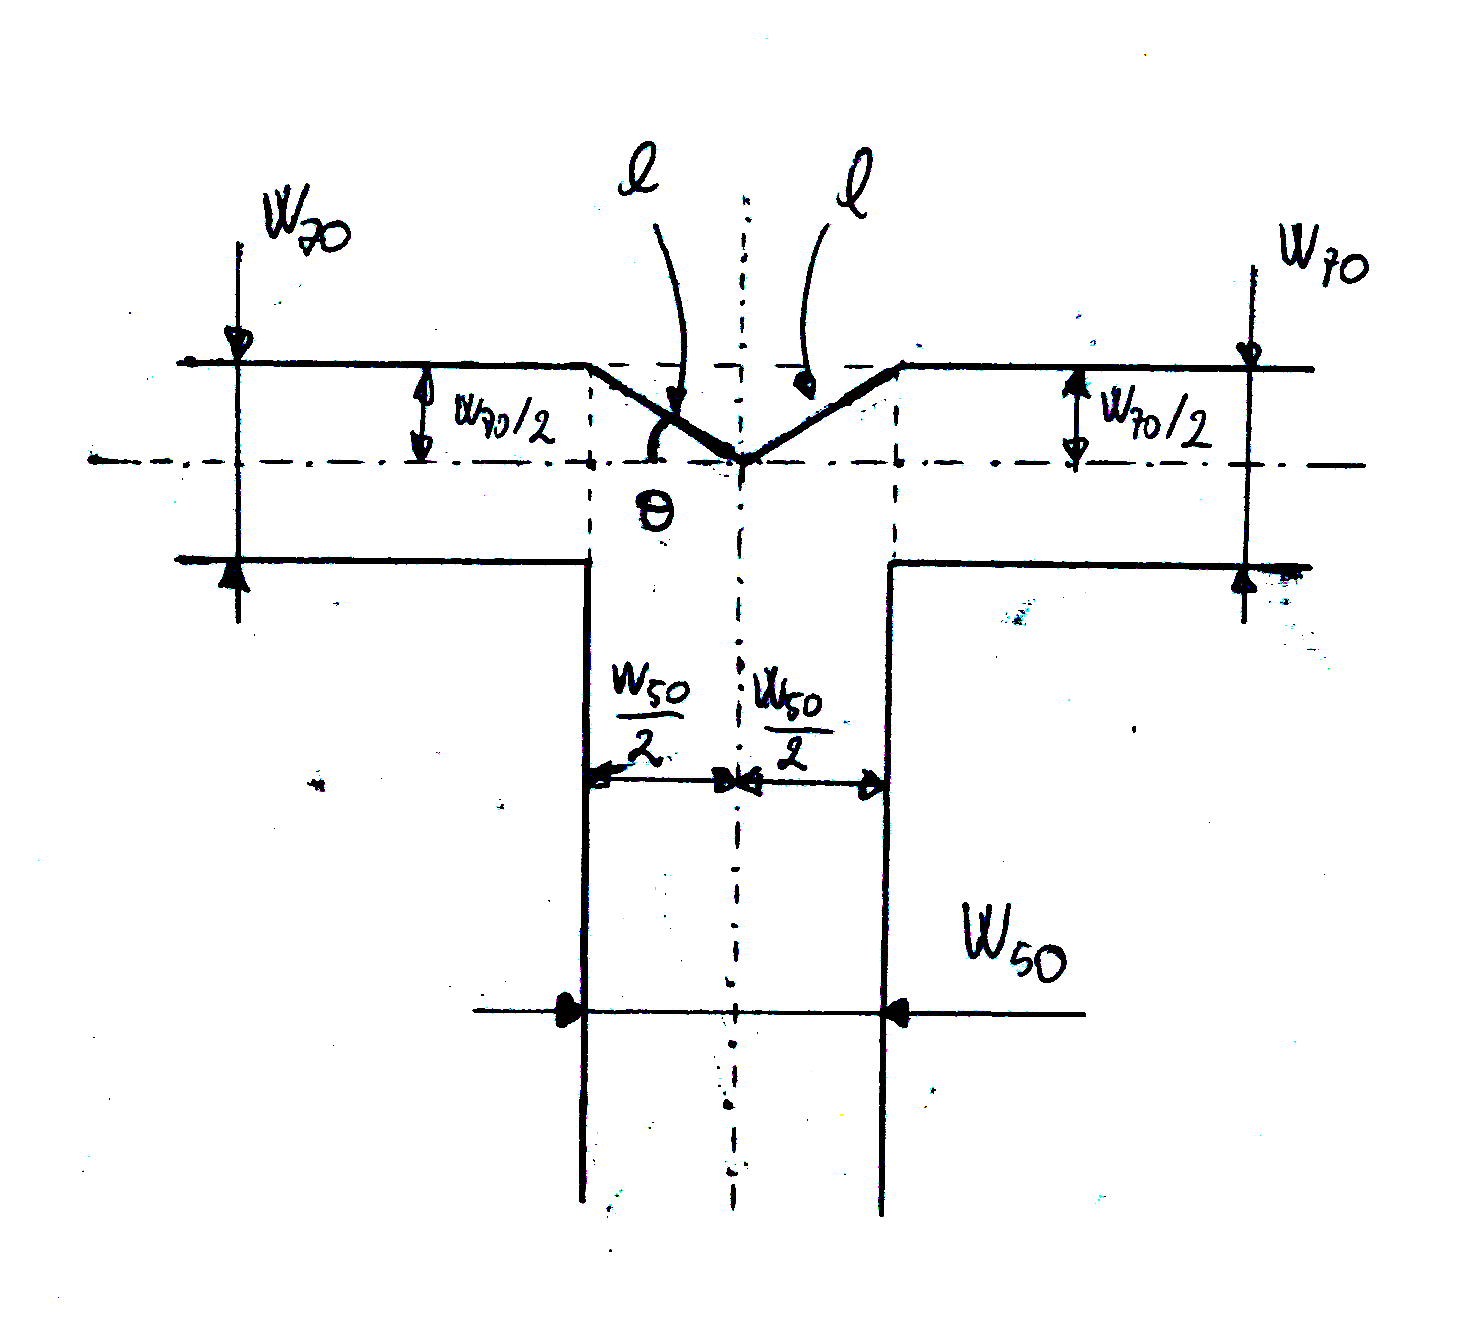
\includegraphics[scale=.4]{A_3dBT}}\quad
	\subfloat[][\emph{5.3dB splitter}]{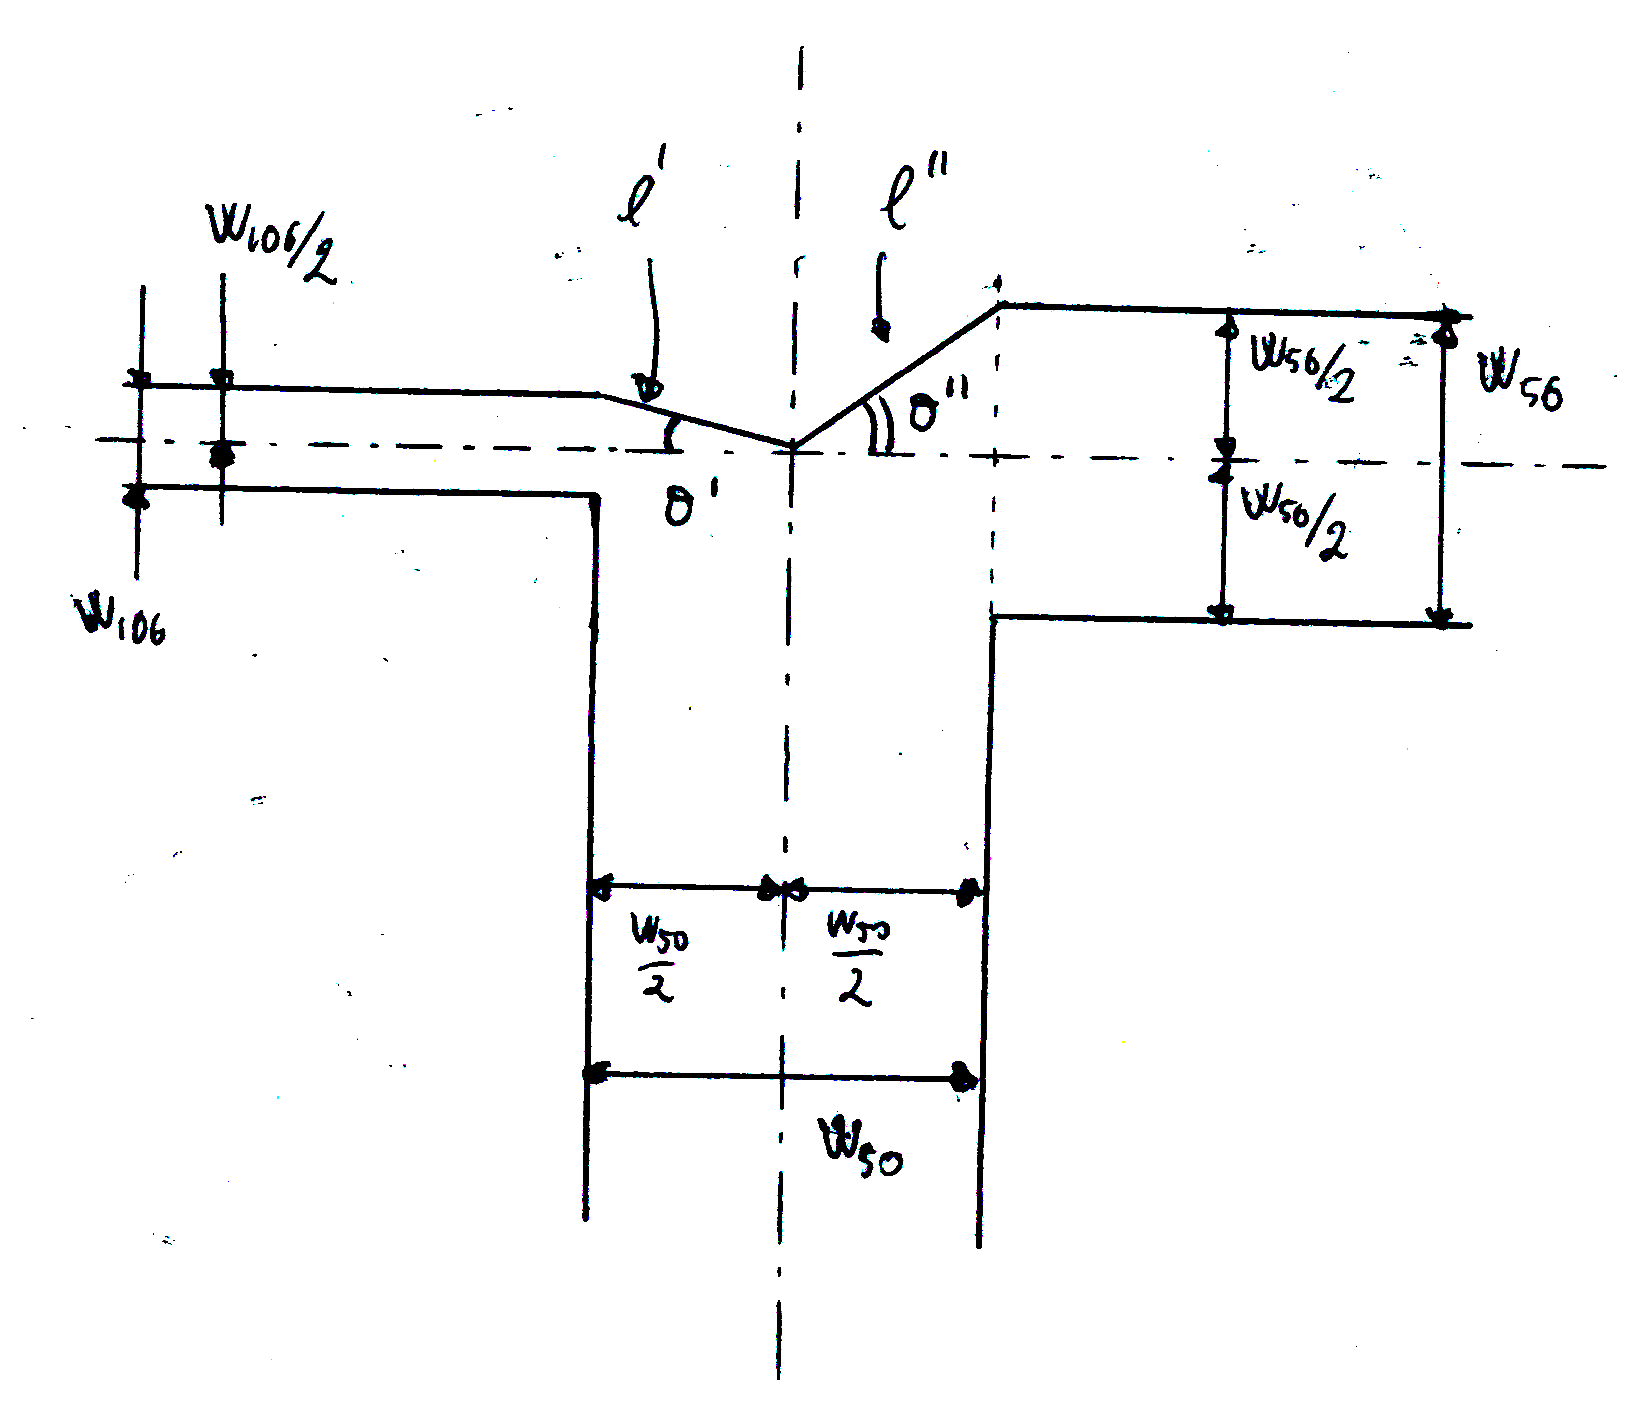
\includegraphics[scale=.35]{A_5dBT}}\\
	\caption{Designed T-junction.}.
	\label{fig:p3_mitered_junctions}
\end{figure}

\newpage
\section{Appendix: input line length dependence}

Our 50$\Omega$ input line has a length of about 35mm. The connection between the transceiver is likely to happen by means of a coaxial cable, whose length would be actually undefined, then it is important to make the array independent on the input line length. Hence, the BFN must be able both to perfectly match the feeding line with the patches and keep the input reflection coefficient low enough (in our case this is mainly accomplished through the 70$\Omega$ quarter wavelength transformers and the 50$\Omega$ bends compensation), whichever the feeding line's length.

To verify the good behaviour of the input matching we propose the simulation outcomes depicted in figure \ref{fig:A_INlineL}, where the input vertical 50$\Omega$ line length has been changed. 

\begin{figure}[H] 
	\centering
	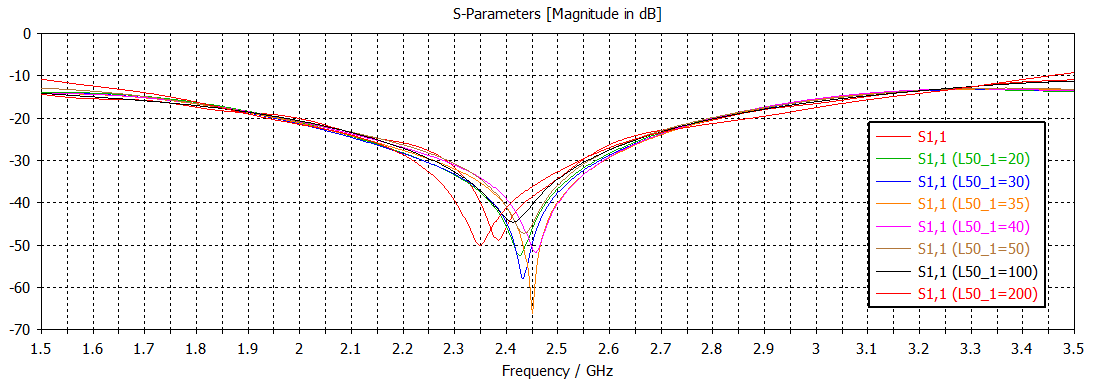
\includegraphics[scale=0.45]{A_length}
	\caption{The input line length has been changed, the measures are expressed in millimetres. System is really sensible to lines longer than 50mm, showing a shift in resonance frequency above that value.}
	\label{fig:A_INlineL}
\end{figure}
